\section{Contribution}

% nous allons trouver un compromis entre le temps d'execution et l'equilibrage de charge
%\begin{frame}
%\centering
%	\vspace{2.2cm}       
%	\Huge 
%	\textbf{Pourquoi \\la réduction des transitions externes \\et\\ l'équilibrage des états \\n'aide pas le model checking ?}	
%\end{frame}

% avant tout, presentons les point de partitions
%tout partition outre les point que la formule n'est pas verifier initialement entrainera un nombre de calcule. les exemples precedents le demontre.

%il peut arriver que les machine ne peuvent pas supporter ces etats par leur nombres
%le mieux est de le surcharger en calcule ou en stockage que les deux en meme temps
\subsection{Points de partitions}
\begin{frame}{Définition}
  \centering
   \begin{columns}
   	\begin{column}{0.8\textwidth}
   		\vspace{-20pt}
   		\begin{figure}				
   			\begin{tikzpicture}		
   			\only<1-1>
   			{
   				\node [inner sep=-10pt]
   				{
   					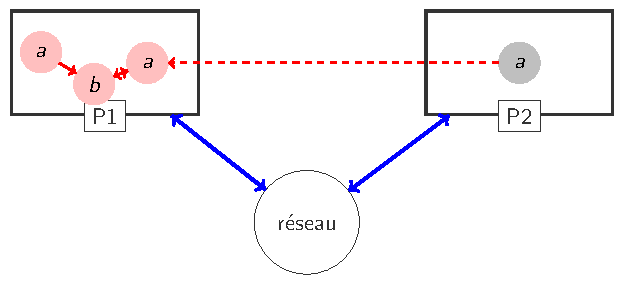
\includegraphics[height=1.2in,width=\columnwidth,trim={0 0 0 0},clip]{resources/benstira/critque1}
   				};              
   			}
   			
   			\node [inner sep=-10pt,visible on=<2->]
   			{
   				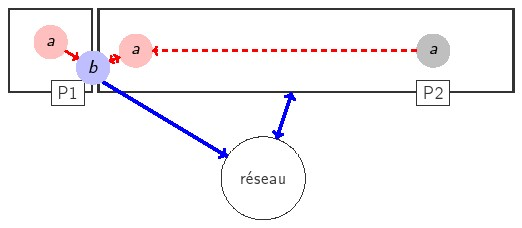
\includegraphics[height=1.2in,width=\columnwidth,trim={0 0 0 0},clip]{resources/pointpartition}
   			};
   		
   			\end{tikzpicture}				
   		\end{figure}
   	\end{column}   	
   \end{columns}

\begin{columns}
	\begin{column}{0.8\textwidth}
		\vspace{15pt}
		\begin{figure}				
			\begin{tikzpicture}	
			\node [inner sep=-10pt,visible on=<3->]
			{
				
\includegraphics[height=1in,width=0.5\columnwidth,trim={0 0 0 0},clip]{resources/pc}
			};			
			\end{tikzpicture}				
		\end{figure}
	\end{column}   	
\end{columns}
\end{frame}

\subsection{Équilibre de Nash}
\begin{frame}{Définition}
\centering
\vspace{-20pt}
\begin{columns}
	\begin{column}{0.3\textwidth}
		\begin{figure}
			\centering
			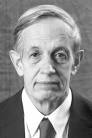
\includegraphics[width=\linewidth]{resources/nash}
		\end{figure}
		
	\end{column}
	\begin{column}{0.7\textwidth}
		\begin{itemize}
			\item Une situation o\`{u} adopte la meilleure réponse du choix des autres.
			\item Il lui a valu le  \textbf{Prix Nobel}  d'économie en 1994.
			%L'existence d'un équilibre n'implique pas que celui-ci soit nécessairement optimal
		\end{itemize}
	\centering
	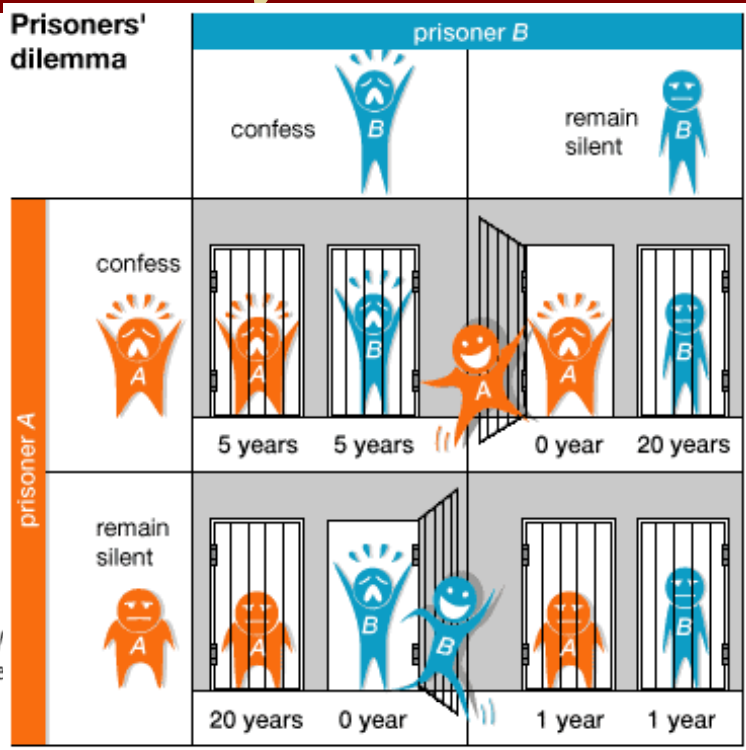
\includegraphics[width=0.5\linewidth]{resources/prisonier}
	\end{column}   	
\end{columns}
\end{frame}


%nous comptons utiliser cette philosophie pour equilibrer le temps de la verification tout en degradant le stockage

\subsection{Stratégie de Distribution}
\begin{frame}{title subsection}
\centering
\vspace{-20pt}
\begin{columns}
	\begin{column}{1\textwidth}
		\begin{figure}
			\centering
			\begin{tikzpicture}	
			\node [inner sep=-10pt,visible on=<1-1>]
			{
				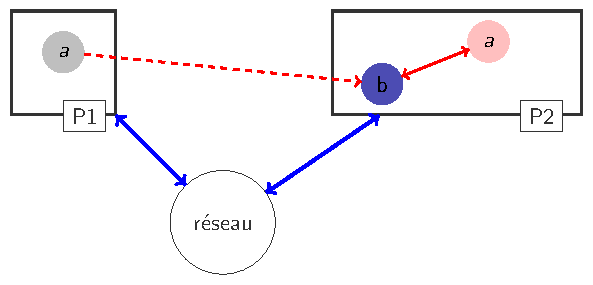
\includegraphics[width=\columnwidth,trim={0 0 0 0},clip]{resources/d1}
			};	
			\node [inner sep=-10pt,visible on=<2-2>]
			{
				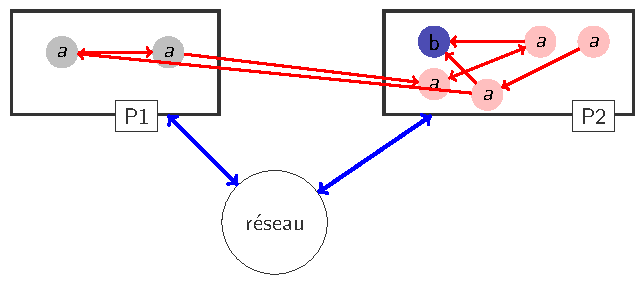
\includegraphics[width=\columnwidth,trim={0 0 0 0},clip]{resources/d2}
			};			
			 
			 \node [inner sep=-10pt,visible on=<3-3>]
			 {
			 	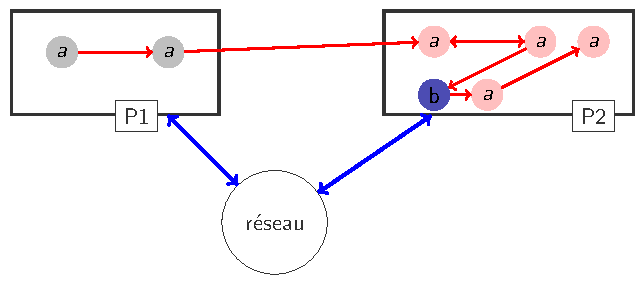
\includegraphics[width=\columnwidth,trim={0 0 0 0},clip]{resources/d3}
			 };	
		 
		 	\node [inner sep=-10pt,visible on=<4-4>]
		 	{
		 		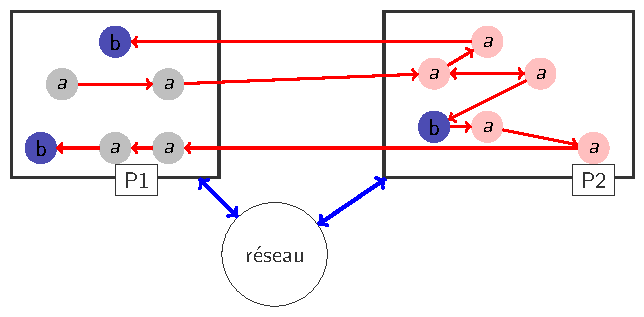
\includegraphics[width=\columnwidth,trim={0 0 0 0},clip]{resources/d5}
		 	};	
	 	
	 	    \node [inner sep=-10pt,visible on=<5-5>]
	 	    {
	 	    	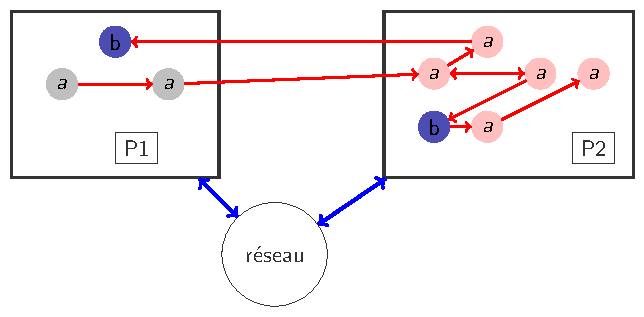
\includegraphics[width=\columnwidth,trim={0 0 0 0},clip]{resources/d4}
	 	    };	
 	    
 	    	\node [inner sep=-10pt,visible on=<6-6>]
 	    	{
 	    		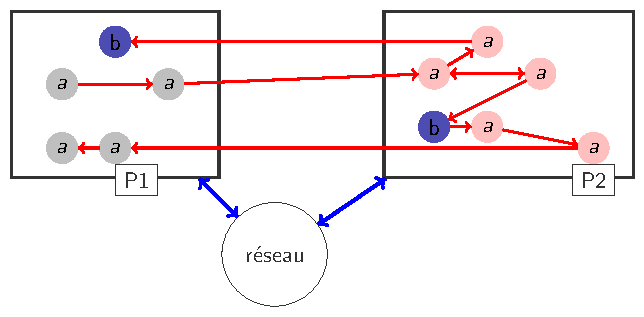
\includegraphics[width=\columnwidth,trim={0 0 0 0},clip]{resources/d6}
 	    	};	
     	
     		\node [inner sep=-10pt,visible on=<7-7>]
     		{
     			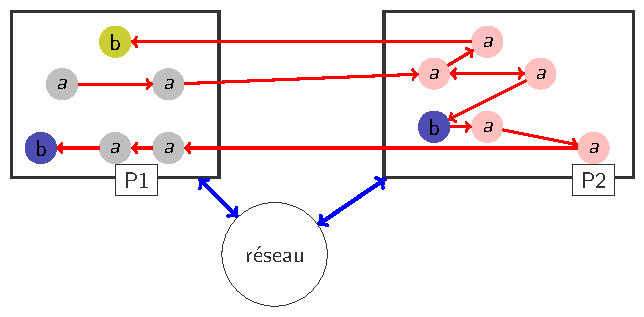
\includegraphics[width=\columnwidth,trim={0 0 0 0},clip]{resources/d7}
     		};	
     	
     		\node [inner sep=-10pt,visible on=<8-8>]
     		{
     			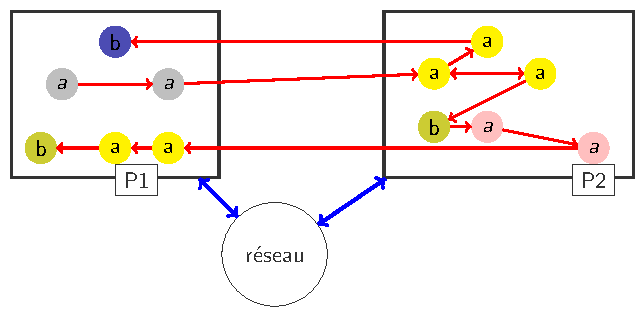
\includegraphics[width=\columnwidth,trim={0 0 0 0},clip]{resources/d8}
     		};	
     	
			\end{tikzpicture}
		\end{figure}		
	\end{column} 
	
\end{columns}
\end{frame}
%nous comptons a realiser une meilleur partion
\subsection{Model checking par déduction}
\begin{frame}{title subsection}
	\begin{block}
	
	\begin{itemize}
		\item Notion de duplicata
		\item Déduit la valeur logique des duplicatas
		\item Minimise le taux de communications
	\end{itemize}
	\end{block}
\end{frame}

%ces deux approche permet d'accelerer le temps de la verification d'une propriete 